\documentclass[twoside]{book}

% Packages required by doxygen
\usepackage{fixltx2e}
\usepackage{calc}
\usepackage{doxygen}
\usepackage[export]{adjustbox} % also loads graphicx
\usepackage{graphicx}
\usepackage[utf8]{inputenc}
\usepackage{makeidx}
\usepackage{multicol}
\usepackage{multirow}
\PassOptionsToPackage{warn}{textcomp}
\usepackage{textcomp}
\usepackage[nointegrals]{wasysym}
\usepackage[table]{xcolor}

% Font selection
\usepackage[T1]{fontenc}
\usepackage[scaled=.90]{helvet}
\usepackage{courier}
\usepackage{amssymb}
\usepackage{sectsty}
\renewcommand{\familydefault}{\sfdefault}
\allsectionsfont{%
  \fontseries{bc}\selectfont%
  \color{darkgray}%
}
\renewcommand{\DoxyLabelFont}{%
  \fontseries{bc}\selectfont%
  \color{darkgray}%
}
\newcommand{\+}{\discretionary{\mbox{\scriptsize$\hookleftarrow$}}{}{}}

% Page & text layout
\usepackage{geometry}
\geometry{%
  a4paper,%
  top=2.5cm,%
  bottom=2.5cm,%
  left=2.5cm,%
  right=2.5cm%
}
\tolerance=750
\hfuzz=15pt
\hbadness=750
\setlength{\emergencystretch}{15pt}
\setlength{\parindent}{0cm}
\setlength{\parskip}{3ex plus 2ex minus 2ex}
\makeatletter
\renewcommand{\paragraph}{%
  \@startsection{paragraph}{4}{0ex}{-1.0ex}{1.0ex}{%
    \normalfont\normalsize\bfseries\SS@parafont%
  }%
}
\renewcommand{\subparagraph}{%
  \@startsection{subparagraph}{5}{0ex}{-1.0ex}{1.0ex}{%
    \normalfont\normalsize\bfseries\SS@subparafont%
  }%
}
\makeatother

% Headers & footers
\usepackage{fancyhdr}
\pagestyle{fancyplain}
\fancyhead[LE]{\fancyplain{}{\bfseries\thepage}}
\fancyhead[CE]{\fancyplain{}{}}
\fancyhead[RE]{\fancyplain{}{\bfseries\leftmark}}
\fancyhead[LO]{\fancyplain{}{\bfseries\rightmark}}
\fancyhead[CO]{\fancyplain{}{}}
\fancyhead[RO]{\fancyplain{}{\bfseries\thepage}}
\fancyfoot[LE]{\fancyplain{}{}}
\fancyfoot[CE]{\fancyplain{}{}}
\fancyfoot[RE]{\fancyplain{}{\bfseries\scriptsize Generated by Doxygen }}
\fancyfoot[LO]{\fancyplain{}{\bfseries\scriptsize Generated by Doxygen }}
\fancyfoot[CO]{\fancyplain{}{}}
\fancyfoot[RO]{\fancyplain{}{}}
\renewcommand{\footrulewidth}{0.4pt}
\renewcommand{\chaptermark}[1]{%
  \markboth{#1}{}%
}
\renewcommand{\sectionmark}[1]{%
  \markright{\thesection\ #1}%
}

% Indices & bibliography
\usepackage{natbib}
\usepackage[titles]{tocloft}
\setcounter{tocdepth}{3}
\setcounter{secnumdepth}{5}
\makeindex

% Hyperlinks (required, but should be loaded last)
\usepackage{ifpdf}
\ifpdf
  \usepackage[pdftex,pagebackref=true]{hyperref}
\else
  \usepackage[ps2pdf,pagebackref=true]{hyperref}
\fi
\hypersetup{%
  colorlinks=true,%
  linkcolor=blue,%
  citecolor=blue,%
  unicode%
}

% Custom commands
\newcommand{\clearemptydoublepage}{%
  \newpage{\pagestyle{empty}\cleardoublepage}%
}

\usepackage{caption}
\captionsetup{labelsep=space,justification=centering,font={bf},singlelinecheck=off,skip=4pt,position=top}

%===== C O N T E N T S =====

\begin{document}

% Titlepage & ToC
\hypersetup{pageanchor=false,
             bookmarksnumbered=true,
             pdfencoding=unicode
            }
\pagenumbering{alph}
\begin{titlepage}
\vspace*{7cm}
\begin{center}%
{\Large My Project }\\
\vspace*{1cm}
{\large Generated by Doxygen 1.8.13}\\
\end{center}
\end{titlepage}
\clearemptydoublepage
\pagenumbering{roman}
\tableofcontents
\clearemptydoublepage
\pagenumbering{arabic}
\hypersetup{pageanchor=true}

%--- Begin generated contents ---
\chapter{Class Index}
\section{Class List}
Here are the classes, structs, unions and interfaces with brief descriptions\+:\begin{DoxyCompactList}
\item\contentsline{section}{\hyperlink{structPersonnage}{Personnage} }{\pageref{structPersonnage}}{}
\item\contentsline{section}{\hyperlink{structpersonnage}{personnage} \\*Struct for personnage }{\pageref{structpersonnage}}{}
\item\contentsline{section}{\hyperlink{structPersonnage2}{Personnage2} }{\pageref{structPersonnage2}}{}
\end{DoxyCompactList}

\chapter{File Index}
\section{File List}
Here is a list of all files with brief descriptions\+:\begin{DoxyCompactList}
\item\contentsline{section}{\hyperlink{2eme_01personnage_8h}{2eme personnage.\+h} }{\pageref{2eme_01personnage_8h}}{}
\item\contentsline{section}{\hyperlink{init__personnage_8c}{init\+\_\+personnage.\+c} }{\pageref{init__personnage_8c}}{}
\item\contentsline{section}{\hyperlink{init__personnage2_8c}{init\+\_\+personnage2.\+c} }{\pageref{init__personnage2_8c}}{}
\item\contentsline{section}{\hyperlink{partage__ecran_8c}{partage\+\_\+ecran.\+c} \\*Testing program }{\pageref{partage__ecran_8c}}{}
\item\contentsline{section}{\hyperlink{partage__ecran_8h}{partage\+\_\+ecran.\+h} }{\pageref{partage__ecran_8h}}{}
\item\contentsline{section}{\hyperlink{personnage_8c}{personnage.\+c} \\*Testing program }{\pageref{personnage_8c}}{}
\item\contentsline{section}{\hyperlink{personnage_8h}{personnage.\+h} }{\pageref{personnage_8h}}{}
\item\contentsline{section}{\hyperlink{personnage2_8c}{personnage2.\+c} \\*Testing program }{\pageref{personnage2_8c}}{}
\end{DoxyCompactList}

\chapter{Class Documentation}
\hypertarget{structPersonnage}{}\section{Personnage Struct Reference}
\label{structPersonnage}\index{Personnage@{Personnage}}


{\ttfamily \#include $<$personnage.\+h$>$}

\subsection*{Public Attributes}
\begin{DoxyCompactItemize}
\item 
int \hyperlink{structPersonnage_aed98af55dd1a3b21c5a446713061b67e}{x}
\item 
int \hyperlink{structPersonnage_a4fdc0728efe8d50059d81a7672c86555}{y}
\item 
int \hyperlink{structPersonnage_ab963d6c6eefa127548925d238119c89d}{vx}
\item 
int \hyperlink{structPersonnage_abe7e4fcd3b7657014b2f00126c506773}{vy}
\item 
S\+D\+L\+\_\+\+Surface $\ast$$\ast$ \hyperlink{structPersonnage_a467b1cc114334f7fb81ae69735d3e550}{screen}
\item 
S\+D\+L\+\_\+\+Surface $\ast$ \hyperlink{structPersonnage_ac93a37ebe619525ecd941dafe6ccff7c}{image}
\item 
S\+D\+L\+\_\+\+Surface $\ast$ \hyperlink{structPersonnage_ad54b53de74e952208e3bf3e174fbe6f4}{image2}
\item 
S\+D\+L\+\_\+\+Rect \hyperlink{structPersonnage_abad4e4ba6f919236ccb16b123a862b63}{position}
\item 
S\+D\+L\+\_\+\+Rect \hyperlink{structPersonnage_ab8784d8fd3ed53b0d45b042f6c7021ca}{clips} \mbox{[}00\mbox{]}
\item 
S\+D\+L\+\_\+\+Rect \hyperlink{structPersonnage_a566f023dd52366a0aac09cc1c9166548}{clips2} \mbox{[}00\mbox{]}
\item 
float \hyperlink{structPersonnage_a6a90db01fde50e7af3ab603ce7e4d78d}{frame}
\end{DoxyCompactItemize}


\subsection{Member Data Documentation}
\mbox{\Hypertarget{structPersonnage_ab8784d8fd3ed53b0d45b042f6c7021ca}\label{structPersonnage_ab8784d8fd3ed53b0d45b042f6c7021ca}} 
\index{Personnage@{Personnage}!clips@{clips}}
\index{clips@{clips}!Personnage@{Personnage}}
\subsubsection{\texorpdfstring{clips}{clips}}
{\footnotesize\ttfamily S\+D\+L\+\_\+\+Rect Personnage\+::clips\mbox{[}00\mbox{]}}

\mbox{\Hypertarget{structPersonnage_a566f023dd52366a0aac09cc1c9166548}\label{structPersonnage_a566f023dd52366a0aac09cc1c9166548}} 
\index{Personnage@{Personnage}!clips2@{clips2}}
\index{clips2@{clips2}!Personnage@{Personnage}}
\subsubsection{\texorpdfstring{clips2}{clips2}}
{\footnotesize\ttfamily S\+D\+L\+\_\+\+Rect Personnage\+::clips2\mbox{[}00\mbox{]}}

\mbox{\Hypertarget{structPersonnage_a6a90db01fde50e7af3ab603ce7e4d78d}\label{structPersonnage_a6a90db01fde50e7af3ab603ce7e4d78d}} 
\index{Personnage@{Personnage}!frame@{frame}}
\index{frame@{frame}!Personnage@{Personnage}}
\subsubsection{\texorpdfstring{frame}{frame}}
{\footnotesize\ttfamily float Personnage\+::frame}

\mbox{\Hypertarget{structPersonnage_ac93a37ebe619525ecd941dafe6ccff7c}\label{structPersonnage_ac93a37ebe619525ecd941dafe6ccff7c}} 
\index{Personnage@{Personnage}!image@{image}}
\index{image@{image}!Personnage@{Personnage}}
\subsubsection{\texorpdfstring{image}{image}}
{\footnotesize\ttfamily S\+D\+L\+\_\+\+Surface $\ast$ Personnage\+::image}

\mbox{\Hypertarget{structPersonnage_ad54b53de74e952208e3bf3e174fbe6f4}\label{structPersonnage_ad54b53de74e952208e3bf3e174fbe6f4}} 
\index{Personnage@{Personnage}!image2@{image2}}
\index{image2@{image2}!Personnage@{Personnage}}
\subsubsection{\texorpdfstring{image2}{image2}}
{\footnotesize\ttfamily S\+D\+L\+\_\+\+Surface $\ast$ Personnage\+::image2}

\mbox{\Hypertarget{structPersonnage_abad4e4ba6f919236ccb16b123a862b63}\label{structPersonnage_abad4e4ba6f919236ccb16b123a862b63}} 
\index{Personnage@{Personnage}!position@{position}}
\index{position@{position}!Personnage@{Personnage}}
\subsubsection{\texorpdfstring{position}{position}}
{\footnotesize\ttfamily S\+D\+L\+\_\+\+Rect Personnage\+::position}

\mbox{\Hypertarget{structPersonnage_a467b1cc114334f7fb81ae69735d3e550}\label{structPersonnage_a467b1cc114334f7fb81ae69735d3e550}} 
\index{Personnage@{Personnage}!screen@{screen}}
\index{screen@{screen}!Personnage@{Personnage}}
\subsubsection{\texorpdfstring{screen}{screen}}
{\footnotesize\ttfamily S\+D\+L\+\_\+\+Surface$\ast$$\ast$ Personnage\+::screen}

\mbox{\Hypertarget{structPersonnage_ab963d6c6eefa127548925d238119c89d}\label{structPersonnage_ab963d6c6eefa127548925d238119c89d}} 
\index{Personnage@{Personnage}!vx@{vx}}
\index{vx@{vx}!Personnage@{Personnage}}
\subsubsection{\texorpdfstring{vx}{vx}}
{\footnotesize\ttfamily int Personnage\+::vx}

\mbox{\Hypertarget{structPersonnage_abe7e4fcd3b7657014b2f00126c506773}\label{structPersonnage_abe7e4fcd3b7657014b2f00126c506773}} 
\index{Personnage@{Personnage}!vy@{vy}}
\index{vy@{vy}!Personnage@{Personnage}}
\subsubsection{\texorpdfstring{vy}{vy}}
{\footnotesize\ttfamily int Personnage\+::vy}

\mbox{\Hypertarget{structPersonnage_aed98af55dd1a3b21c5a446713061b67e}\label{structPersonnage_aed98af55dd1a3b21c5a446713061b67e}} 
\index{Personnage@{Personnage}!x@{x}}
\index{x@{x}!Personnage@{Personnage}}
\subsubsection{\texorpdfstring{x}{x}}
{\footnotesize\ttfamily int Personnage\+::x}

\mbox{\Hypertarget{structPersonnage_a4fdc0728efe8d50059d81a7672c86555}\label{structPersonnage_a4fdc0728efe8d50059d81a7672c86555}} 
\index{Personnage@{Personnage}!y@{y}}
\index{y@{y}!Personnage@{Personnage}}
\subsubsection{\texorpdfstring{y}{y}}
{\footnotesize\ttfamily int Personnage\+::y}



The documentation for this struct was generated from the following file\+:\begin{DoxyCompactItemize}
\item 
\hyperlink{personnage_8h}{personnage.\+h}\end{DoxyCompactItemize}

\hypertarget{structpersonnage}{}\section{personnage Struct Reference}
\label{structpersonnage}\index{personnage@{personnage}}


struct for personnage  




{\ttfamily \#include $<$personnage.\+h$>$}



\subsection{Detailed Description}
struct for personnage 

\begin{DoxyAuthor}{Author}
phunyuka 
\end{DoxyAuthor}


The documentation for this struct was generated from the following file\+:\begin{DoxyCompactItemize}
\item 
\hyperlink{personnage_8h}{personnage.\+h}\end{DoxyCompactItemize}

\hypertarget{structPersonnage2}{}\section{Personnage2 Struct Reference}
\label{structPersonnage2}\index{Personnage2@{Personnage2}}


{\ttfamily \#include $<$2eme personnage.\+h$>$}

\subsection*{Public Attributes}
\begin{DoxyCompactItemize}
\item 
int \hyperlink{structPersonnage2_ae1441c9154226c8f192692a60640ea6c}{x}
\item 
int \hyperlink{structPersonnage2_ac955392c8e030015e46517244e5987bd}{y}
\item 
int \hyperlink{structPersonnage2_aaf15cd6e8f9e8f75fcf079b8708f8ca3}{vx}
\item 
int \hyperlink{structPersonnage2_ab90fadbadf36db5de02082c7a2ee1aba}{vy}
\item 
S\+D\+L\+\_\+\+Surface $\ast$$\ast$ \hyperlink{structPersonnage2_a9ba0907380a892c9bc00b01cab744baf}{screen}
\item 
S\+D\+L\+\_\+\+Surface $\ast$ \hyperlink{structPersonnage2_a8b388edbf0064274aaee5c45b926b54b}{image}
\item 
S\+D\+L\+\_\+\+Surface $\ast$ \hyperlink{structPersonnage2_a185520d9aed81f2a5f1c157a2965b334}{image2}
\item 
S\+D\+L\+\_\+\+Rect \hyperlink{structPersonnage2_af34f6010776bf89a19c2a1af1400e885}{position}
\item 
S\+D\+L\+\_\+\+Rect \hyperlink{structPersonnage2_a70e37d07b50f6d4f576f31a968545afe}{clips} \mbox{[}00\mbox{]}
\item 
S\+D\+L\+\_\+\+Rect \hyperlink{structPersonnage2_aca4b0202064d5f466b3b3a6ba1e009b5}{clips2} \mbox{[}00\mbox{]}
\item 
float \hyperlink{structPersonnage2_a4256be539bf8145469f5d7189c768e9b}{frame}
\end{DoxyCompactItemize}


\subsection{Member Data Documentation}
\mbox{\Hypertarget{structPersonnage2_a70e37d07b50f6d4f576f31a968545afe}\label{structPersonnage2_a70e37d07b50f6d4f576f31a968545afe}} 
\index{Personnage2@{Personnage2}!clips@{clips}}
\index{clips@{clips}!Personnage2@{Personnage2}}
\subsubsection{\texorpdfstring{clips}{clips}}
{\footnotesize\ttfamily S\+D\+L\+\_\+\+Rect Personnage2\+::clips\mbox{[}00\mbox{]}}

\mbox{\Hypertarget{structPersonnage2_aca4b0202064d5f466b3b3a6ba1e009b5}\label{structPersonnage2_aca4b0202064d5f466b3b3a6ba1e009b5}} 
\index{Personnage2@{Personnage2}!clips2@{clips2}}
\index{clips2@{clips2}!Personnage2@{Personnage2}}
\subsubsection{\texorpdfstring{clips2}{clips2}}
{\footnotesize\ttfamily S\+D\+L\+\_\+\+Rect Personnage2\+::clips2\mbox{[}00\mbox{]}}

\mbox{\Hypertarget{structPersonnage2_a4256be539bf8145469f5d7189c768e9b}\label{structPersonnage2_a4256be539bf8145469f5d7189c768e9b}} 
\index{Personnage2@{Personnage2}!frame@{frame}}
\index{frame@{frame}!Personnage2@{Personnage2}}
\subsubsection{\texorpdfstring{frame}{frame}}
{\footnotesize\ttfamily float Personnage2\+::frame}

\mbox{\Hypertarget{structPersonnage2_a8b388edbf0064274aaee5c45b926b54b}\label{structPersonnage2_a8b388edbf0064274aaee5c45b926b54b}} 
\index{Personnage2@{Personnage2}!image@{image}}
\index{image@{image}!Personnage2@{Personnage2}}
\subsubsection{\texorpdfstring{image}{image}}
{\footnotesize\ttfamily S\+D\+L\+\_\+\+Surface $\ast$ Personnage2\+::image}

\mbox{\Hypertarget{structPersonnage2_a185520d9aed81f2a5f1c157a2965b334}\label{structPersonnage2_a185520d9aed81f2a5f1c157a2965b334}} 
\index{Personnage2@{Personnage2}!image2@{image2}}
\index{image2@{image2}!Personnage2@{Personnage2}}
\subsubsection{\texorpdfstring{image2}{image2}}
{\footnotesize\ttfamily S\+D\+L\+\_\+\+Surface $\ast$ Personnage2\+::image2}

\mbox{\Hypertarget{structPersonnage2_af34f6010776bf89a19c2a1af1400e885}\label{structPersonnage2_af34f6010776bf89a19c2a1af1400e885}} 
\index{Personnage2@{Personnage2}!position@{position}}
\index{position@{position}!Personnage2@{Personnage2}}
\subsubsection{\texorpdfstring{position}{position}}
{\footnotesize\ttfamily S\+D\+L\+\_\+\+Rect Personnage2\+::position}

\mbox{\Hypertarget{structPersonnage2_a9ba0907380a892c9bc00b01cab744baf}\label{structPersonnage2_a9ba0907380a892c9bc00b01cab744baf}} 
\index{Personnage2@{Personnage2}!screen@{screen}}
\index{screen@{screen}!Personnage2@{Personnage2}}
\subsubsection{\texorpdfstring{screen}{screen}}
{\footnotesize\ttfamily S\+D\+L\+\_\+\+Surface$\ast$$\ast$ Personnage2\+::screen}

\mbox{\Hypertarget{structPersonnage2_aaf15cd6e8f9e8f75fcf079b8708f8ca3}\label{structPersonnage2_aaf15cd6e8f9e8f75fcf079b8708f8ca3}} 
\index{Personnage2@{Personnage2}!vx@{vx}}
\index{vx@{vx}!Personnage2@{Personnage2}}
\subsubsection{\texorpdfstring{vx}{vx}}
{\footnotesize\ttfamily int Personnage2\+::vx}

\mbox{\Hypertarget{structPersonnage2_ab90fadbadf36db5de02082c7a2ee1aba}\label{structPersonnage2_ab90fadbadf36db5de02082c7a2ee1aba}} 
\index{Personnage2@{Personnage2}!vy@{vy}}
\index{vy@{vy}!Personnage2@{Personnage2}}
\subsubsection{\texorpdfstring{vy}{vy}}
{\footnotesize\ttfamily int Personnage2\+::vy}

\mbox{\Hypertarget{structPersonnage2_ae1441c9154226c8f192692a60640ea6c}\label{structPersonnage2_ae1441c9154226c8f192692a60640ea6c}} 
\index{Personnage2@{Personnage2}!x@{x}}
\index{x@{x}!Personnage2@{Personnage2}}
\subsubsection{\texorpdfstring{x}{x}}
{\footnotesize\ttfamily int Personnage2\+::x}

\mbox{\Hypertarget{structPersonnage2_ac955392c8e030015e46517244e5987bd}\label{structPersonnage2_ac955392c8e030015e46517244e5987bd}} 
\index{Personnage2@{Personnage2}!y@{y}}
\index{y@{y}!Personnage2@{Personnage2}}
\subsubsection{\texorpdfstring{y}{y}}
{\footnotesize\ttfamily int Personnage2\+::y}



The documentation for this struct was generated from the following file\+:\begin{DoxyCompactItemize}
\item 
\hyperlink{2eme_01personnage_8h}{2eme personnage.\+h}\end{DoxyCompactItemize}

\chapter{File Documentation}
\hypertarget{2eme_01personnage_8h}{}\section{2eme personnage.\+h File Reference}
\label{2eme_01personnage_8h}\index{2eme personnage.\+h@{2eme personnage.\+h}}
{\ttfamily \#include $<$S\+D\+L/\+S\+D\+L.\+h$>$}\newline
{\ttfamily \#include $<$S\+D\+L/\+S\+D\+L\+\_\+image.\+h$>$}\newline
Include dependency graph for 2eme personnage.\+h\+:
\nopagebreak
\begin{figure}[H]
\begin{center}
\leavevmode
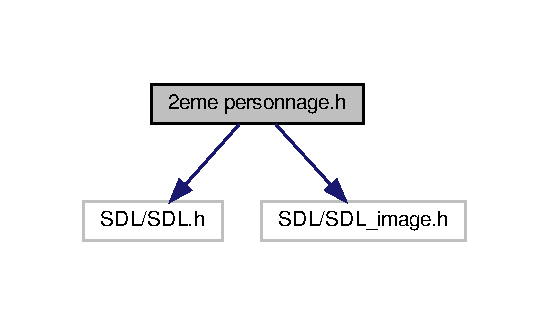
\includegraphics[width=264pt]{2eme_01personnage_8h__incl}
\end{center}
\end{figure}
\subsection*{Classes}
\begin{DoxyCompactItemize}
\item 
struct \hyperlink{structPersonnage2}{Personnage2}
\end{DoxyCompactItemize}
\subsection*{Typedefs}
\begin{DoxyCompactItemize}
\item 
typedef struct \hyperlink{structPersonnage2}{Personnage2} \hyperlink{2eme_01personnage_8h_a14182d75f63f296c0c992296e56a37e1}{Player}
\end{DoxyCompactItemize}
\subsection*{Functions}
\begin{DoxyCompactItemize}
\item 
void \hyperlink{2eme_01personnage_8h_a31593ba691d553fc2777f58c6935c29a}{Personnage\+\_\+\+Init2} (\hyperlink{2eme_01personnage_8h_a14182d75f63f296c0c992296e56a37e1}{Player} $\ast$p)
\item 
void \hyperlink{2eme_01personnage_8h_a40ea1b6da343bdd7899da24e4fbf804d}{Personnage\+\_\+\+Render2} (\hyperlink{2eme_01personnage_8h_a14182d75f63f296c0c992296e56a37e1}{Player} $\ast$p, S\+D\+L\+\_\+\+Rect r, S\+D\+L\+\_\+\+Surface $\ast$$\ast$screen)
\end{DoxyCompactItemize}


\subsection{Typedef Documentation}
\mbox{\Hypertarget{2eme_01personnage_8h_a14182d75f63f296c0c992296e56a37e1}\label{2eme_01personnage_8h_a14182d75f63f296c0c992296e56a37e1}} 
\index{2eme personnage.\+h@{2eme personnage.\+h}!Player@{Player}}
\index{Player@{Player}!2eme personnage.\+h@{2eme personnage.\+h}}
\subsubsection{\texorpdfstring{Player}{Player}}
{\footnotesize\ttfamily typedef struct \hyperlink{structPersonnage2}{Personnage2}  \hyperlink{2eme_01personnage_8h_a14182d75f63f296c0c992296e56a37e1}{Player}}



\subsection{Function Documentation}
\mbox{\Hypertarget{2eme_01personnage_8h_a31593ba691d553fc2777f58c6935c29a}\label{2eme_01personnage_8h_a31593ba691d553fc2777f58c6935c29a}} 
\index{2eme personnage.\+h@{2eme personnage.\+h}!Personnage\+\_\+\+Init2@{Personnage\+\_\+\+Init2}}
\index{Personnage\+\_\+\+Init2@{Personnage\+\_\+\+Init2}!2eme personnage.\+h@{2eme personnage.\+h}}
\subsubsection{\texorpdfstring{Personnage\+\_\+\+Init2()}{Personnage\_Init2()}}
{\footnotesize\ttfamily void Personnage\+\_\+\+Init2 (\begin{DoxyParamCaption}\item[{\hyperlink{2eme_01personnage_8h_a14182d75f63f296c0c992296e56a37e1}{Player} $\ast$}]{p }\end{DoxyParamCaption})}

\mbox{\Hypertarget{2eme_01personnage_8h_a40ea1b6da343bdd7899da24e4fbf804d}\label{2eme_01personnage_8h_a40ea1b6da343bdd7899da24e4fbf804d}} 
\index{2eme personnage.\+h@{2eme personnage.\+h}!Personnage\+\_\+\+Render2@{Personnage\+\_\+\+Render2}}
\index{Personnage\+\_\+\+Render2@{Personnage\+\_\+\+Render2}!2eme personnage.\+h@{2eme personnage.\+h}}
\subsubsection{\texorpdfstring{Personnage\+\_\+\+Render2()}{Personnage\_Render2()}}
{\footnotesize\ttfamily void Personnage\+\_\+\+Render2 (\begin{DoxyParamCaption}\item[{\hyperlink{2eme_01personnage_8h_a14182d75f63f296c0c992296e56a37e1}{Player} $\ast$}]{p,  }\item[{S\+D\+L\+\_\+\+Rect}]{r,  }\item[{S\+D\+L\+\_\+\+Surface $\ast$$\ast$}]{screen }\end{DoxyParamCaption})}


\hypertarget{init__personnage_8c}{}\section{init\+\_\+personnage.\+c File Reference}
\label{init__personnage_8c}\index{init\+\_\+personnage.\+c@{init\+\_\+personnage.\+c}}
{\ttfamily \#include $<$S\+D\+L/\+S\+D\+L.\+h$>$}\newline
{\ttfamily \#include $<$S\+D\+L/\+S\+D\+L\+\_\+image.\+h$>$}\newline
{\ttfamily \#include \char`\"{}personnage.\+h\char`\"{}}\newline
Include dependency graph for init\+\_\+personnage.\+c\+:
\nopagebreak
\begin{figure}[H]
\begin{center}
\leavevmode
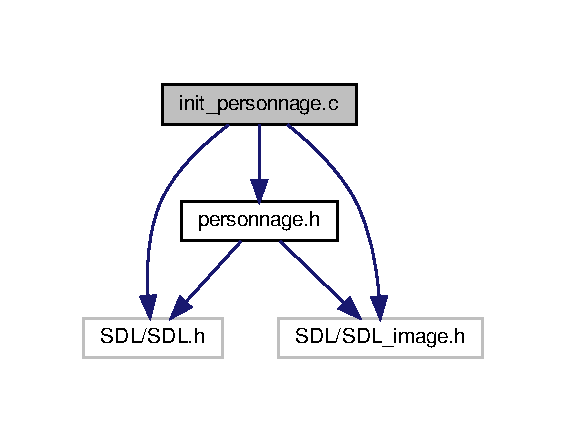
\includegraphics[width=272pt]{init__personnage_8c__incl}
\end{center}
\end{figure}
\subsection*{Functions}
\begin{DoxyCompactItemize}
\item 
void \hyperlink{init__personnage_8c_aea858edd1e8f6fcf5c2f55e455ba63e2}{Personnage\+\_\+\+Init} (\hyperlink{structPersonnage}{Personnage} $\ast$p)
\end{DoxyCompactItemize}


\subsection{Function Documentation}
\mbox{\Hypertarget{init__personnage_8c_aea858edd1e8f6fcf5c2f55e455ba63e2}\label{init__personnage_8c_aea858edd1e8f6fcf5c2f55e455ba63e2}} 
\index{init\+\_\+personnage.\+c@{init\+\_\+personnage.\+c}!Personnage\+\_\+\+Init@{Personnage\+\_\+\+Init}}
\index{Personnage\+\_\+\+Init@{Personnage\+\_\+\+Init}!init\+\_\+personnage.\+c@{init\+\_\+personnage.\+c}}
\subsubsection{\texorpdfstring{Personnage\+\_\+\+Init()}{Personnage\_Init()}}
{\footnotesize\ttfamily void Personnage\+\_\+\+Init (\begin{DoxyParamCaption}\item[{\hyperlink{structPersonnage}{Personnage} $\ast$}]{p }\end{DoxyParamCaption})}


\hypertarget{init__personnage2_8c}{}\section{init\+\_\+personnage2.\+c File Reference}
\label{init__personnage2_8c}\index{init\+\_\+personnage2.\+c@{init\+\_\+personnage2.\+c}}
{\ttfamily \#include $<$S\+D\+L/\+S\+D\+L.\+h$>$}\newline
{\ttfamily \#include $<$S\+D\+L/\+S\+D\+L\+\_\+image.\+h$>$}\newline
{\ttfamily \#include \char`\"{}personnage2.\+h\char`\"{}}\newline
Include dependency graph for init\+\_\+personnage2.\+c\+:
\nopagebreak
\begin{figure}[H]
\begin{center}
\leavevmode
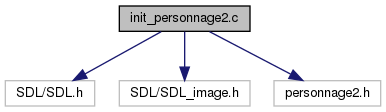
\includegraphics[width=350pt]{init__personnage2_8c__incl}
\end{center}
\end{figure}
\subsection*{Functions}
\begin{DoxyCompactItemize}
\item 
void \hyperlink{init__personnage2_8c_acf6edf8b17437eedee824871caec6bf9}{Personnage\+\_\+\+Init2} (\hyperlink{structPersonnage}{Personnage} $\ast$p)
\end{DoxyCompactItemize}


\subsection{Function Documentation}
\mbox{\Hypertarget{init__personnage2_8c_acf6edf8b17437eedee824871caec6bf9}\label{init__personnage2_8c_acf6edf8b17437eedee824871caec6bf9}} 
\index{init\+\_\+personnage2.\+c@{init\+\_\+personnage2.\+c}!Personnage\+\_\+\+Init2@{Personnage\+\_\+\+Init2}}
\index{Personnage\+\_\+\+Init2@{Personnage\+\_\+\+Init2}!init\+\_\+personnage2.\+c@{init\+\_\+personnage2.\+c}}
\subsubsection{\texorpdfstring{Personnage\+\_\+\+Init2()}{Personnage\_Init2()}}
{\footnotesize\ttfamily void Personnage\+\_\+\+Init2 (\begin{DoxyParamCaption}\item[{\hyperlink{structPersonnage}{Personnage} $\ast$}]{p }\end{DoxyParamCaption})}


\hypertarget{partage__ecran_8c}{}\section{partage\+\_\+ecran.\+c File Reference}
\label{partage__ecran_8c}\index{partage\+\_\+ecran.\+c@{partage\+\_\+ecran.\+c}}


Testing program.  


{\ttfamily \#include $<$stdio.\+h$>$}\newline
{\ttfamily \#include $<$stdlib.\+h$>$}\newline
{\ttfamily \#include $<$S\+D\+L/\+S\+D\+L.\+h$>$}\newline
{\ttfamily \#include $<$S\+D\+L/\+S\+D\+L\+\_\+image.\+h$>$}\newline
{\ttfamily \#include \char`\"{}partage\+\_\+ecran.\+h\char`\"{}}\newline
Include dependency graph for partage\+\_\+ecran.\+c\+:
\nopagebreak
\begin{figure}[H]
\begin{center}
\leavevmode
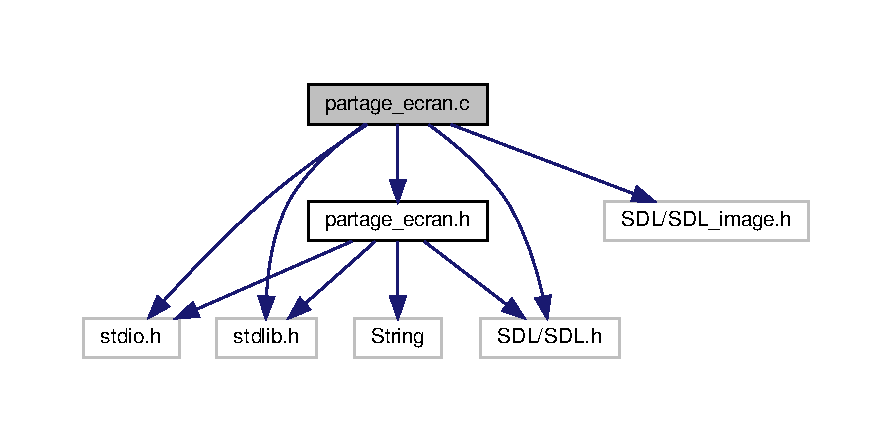
\includegraphics[width=350pt]{partage__ecran_8c__incl}
\end{center}
\end{figure}
\subsection*{Functions}
\begin{DoxyCompactItemize}
\item 
void \hyperlink{partage__ecran_8c_a02fd73d861ef2e4aabb38c0c9ff82947}{init} ()
\item 
void \hyperlink{partage__ecran_8c_ab0dc1c37888f4e354d9187d843e92066}{partage\+\_\+ecran} (S\+D\+L\+\_\+\+Rect poscam1, S\+D\+L\+\_\+\+Rect poscam2, S\+D\+L\+\_\+\+Rect camera1, S\+D\+L\+\_\+\+Rect camera2, S\+D\+L\+\_\+\+Surface $\ast$ecran)
\end{DoxyCompactItemize}


\subsection{Detailed Description}
Testing program. 

\begin{DoxyAuthor}{Author}
C Team 
\end{DoxyAuthor}
\begin{DoxyVersion}{Version}
0.\+1 
\end{DoxyVersion}
\begin{DoxyDate}{Date}
juin 10,2020 testing program 
\end{DoxyDate}


\subsection{Function Documentation}
\mbox{\Hypertarget{partage__ecran_8c_a02fd73d861ef2e4aabb38c0c9ff82947}\label{partage__ecran_8c_a02fd73d861ef2e4aabb38c0c9ff82947}} 
\index{partage\+\_\+ecran.\+c@{partage\+\_\+ecran.\+c}!init@{init}}
\index{init@{init}!partage\+\_\+ecran.\+c@{partage\+\_\+ecran.\+c}}
\subsubsection{\texorpdfstring{init()}{init()}}
{\footnotesize\ttfamily void init (\begin{DoxyParamCaption}{ }\end{DoxyParamCaption})}

\mbox{\Hypertarget{partage__ecran_8c_ab0dc1c37888f4e354d9187d843e92066}\label{partage__ecran_8c_ab0dc1c37888f4e354d9187d843e92066}} 
\index{partage\+\_\+ecran.\+c@{partage\+\_\+ecran.\+c}!partage\+\_\+ecran@{partage\+\_\+ecran}}
\index{partage\+\_\+ecran@{partage\+\_\+ecran}!partage\+\_\+ecran.\+c@{partage\+\_\+ecran.\+c}}
\subsubsection{\texorpdfstring{partage\+\_\+ecran()}{partage\_ecran()}}
{\footnotesize\ttfamily void partage\+\_\+ecran (\begin{DoxyParamCaption}\item[{S\+D\+L\+\_\+\+Rect}]{poscam1,  }\item[{S\+D\+L\+\_\+\+Rect}]{poscam2,  }\item[{S\+D\+L\+\_\+\+Rect}]{camera1,  }\item[{S\+D\+L\+\_\+\+Rect}]{camera2,  }\item[{S\+D\+L\+\_\+\+Surface $\ast$}]{ecran }\end{DoxyParamCaption})}


\hypertarget{partage__ecran_8h}{}\section{partage\+\_\+ecran.\+h File Reference}
\label{partage__ecran_8h}\index{partage\+\_\+ecran.\+h@{partage\+\_\+ecran.\+h}}
{\ttfamily \#include $<$stdio.\+h$>$}\newline
{\ttfamily \#include $<$stdlib.\+h$>$}\newline
{\ttfamily \#include $<$S\+D\+L/\+S\+D\+L.\+h$>$}\newline
{\ttfamily \#include $<$String$>$}\newline
Include dependency graph for partage\+\_\+ecran.\+h\+:
\nopagebreak
\begin{figure}[H]
\begin{center}
\leavevmode
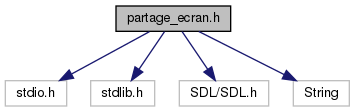
\includegraphics[width=338pt]{partage__ecran_8h__incl}
\end{center}
\end{figure}
This graph shows which files directly or indirectly include this file\+:
\nopagebreak
\begin{figure}[H]
\begin{center}
\leavevmode
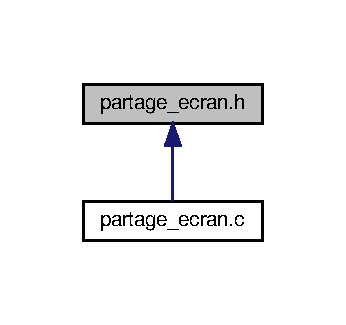
\includegraphics[width=166pt]{partage__ecran_8h__dep__incl}
\end{center}
\end{figure}
\subsection*{Functions}
\begin{DoxyCompactItemize}
\item 
void \hyperlink{partage__ecran_8h_a062734693a34a0833703c41ee67b9aa3}{inti} ()
\item 
void \hyperlink{partage__ecran_8h_ab0dc1c37888f4e354d9187d843e92066}{partage\+\_\+ecran} (S\+D\+L\+\_\+\+Rect poscam1, S\+D\+L\+\_\+\+Rect poscam2, S\+D\+L\+\_\+\+Rect camera1, S\+D\+L\+\_\+\+Rect camera2, S\+D\+L\+\_\+\+Surface $\ast$ecran)
\end{DoxyCompactItemize}


\subsection{Function Documentation}
\mbox{\Hypertarget{partage__ecran_8h_a062734693a34a0833703c41ee67b9aa3}\label{partage__ecran_8h_a062734693a34a0833703c41ee67b9aa3}} 
\index{partage\+\_\+ecran.\+h@{partage\+\_\+ecran.\+h}!inti@{inti}}
\index{inti@{inti}!partage\+\_\+ecran.\+h@{partage\+\_\+ecran.\+h}}
\subsubsection{\texorpdfstring{inti()}{inti()}}
{\footnotesize\ttfamily void inti (\begin{DoxyParamCaption}{ }\end{DoxyParamCaption})}

\mbox{\Hypertarget{partage__ecran_8h_ab0dc1c37888f4e354d9187d843e92066}\label{partage__ecran_8h_ab0dc1c37888f4e354d9187d843e92066}} 
\index{partage\+\_\+ecran.\+h@{partage\+\_\+ecran.\+h}!partage\+\_\+ecran@{partage\+\_\+ecran}}
\index{partage\+\_\+ecran@{partage\+\_\+ecran}!partage\+\_\+ecran.\+h@{partage\+\_\+ecran.\+h}}
\subsubsection{\texorpdfstring{partage\+\_\+ecran()}{partage\_ecran()}}
{\footnotesize\ttfamily void partage\+\_\+ecran (\begin{DoxyParamCaption}\item[{S\+D\+L\+\_\+\+Rect}]{poscam1,  }\item[{S\+D\+L\+\_\+\+Rect}]{poscam2,  }\item[{S\+D\+L\+\_\+\+Rect}]{camera1,  }\item[{S\+D\+L\+\_\+\+Rect}]{camera2,  }\item[{S\+D\+L\+\_\+\+Surface $\ast$}]{ecran }\end{DoxyParamCaption})}


\hypertarget{personnage_8c}{}\section{personnage.\+c File Reference}
\label{personnage_8c}\index{personnage.\+c@{personnage.\+c}}


Testing program.  


{\ttfamily \#include $<$S\+D\+L/\+S\+D\+L.\+h$>$}\newline
{\ttfamily \#include $<$S\+D\+L/\+S\+D\+L\+\_\+image.\+h$>$}\newline
{\ttfamily \#include \char`\"{}personnage.\+h\char`\"{}}\newline
Include dependency graph for personnage.\+c\+:
\nopagebreak
\begin{figure}[H]
\begin{center}
\leavevmode
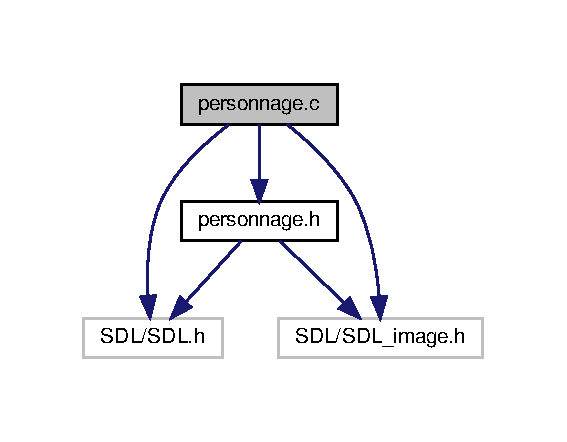
\includegraphics[width=272pt]{personnage_8c__incl}
\end{center}
\end{figure}
\subsection*{Functions}
\begin{DoxyCompactItemize}
\item 
void \hyperlink{personnage_8c_ae662e220210cf8bb89108a9e9f4c3c61}{Personnage\+\_\+\+Render} (\hyperlink{structPersonnage}{Personnage} $\ast$p, S\+D\+L\+\_\+\+Rect r, S\+D\+L\+\_\+\+Surface $\ast$$\ast$screen)
\end{DoxyCompactItemize}


\subsection{Detailed Description}
Testing program. 

\begin{DoxyAuthor}{Author}
C Team 
\end{DoxyAuthor}
\begin{DoxyVersion}{Version}
0.\+1 
\end{DoxyVersion}
\begin{DoxyDate}{Date}
juin 10,2020 testing program 
\end{DoxyDate}


\subsection{Function Documentation}
\mbox{\Hypertarget{personnage_8c_ae662e220210cf8bb89108a9e9f4c3c61}\label{personnage_8c_ae662e220210cf8bb89108a9e9f4c3c61}} 
\index{personnage.\+c@{personnage.\+c}!Personnage\+\_\+\+Render@{Personnage\+\_\+\+Render}}
\index{Personnage\+\_\+\+Render@{Personnage\+\_\+\+Render}!personnage.\+c@{personnage.\+c}}
\subsubsection{\texorpdfstring{Personnage\+\_\+\+Render()}{Personnage\_Render()}}
{\footnotesize\ttfamily void Personnage\+\_\+\+Render (\begin{DoxyParamCaption}\item[{\hyperlink{structPersonnage}{Personnage} $\ast$}]{p,  }\item[{S\+D\+L\+\_\+\+Rect}]{r,  }\item[{S\+D\+L\+\_\+\+Surface $\ast$$\ast$}]{screen }\end{DoxyParamCaption})}


\hypertarget{personnage_8h}{}\section{personnage.\+h File Reference}
\label{personnage_8h}\index{personnage.\+h@{personnage.\+h}}
{\ttfamily \#include $<$S\+D\+L/\+S\+D\+L.\+h$>$}\newline
{\ttfamily \#include $<$S\+D\+L/\+S\+D\+L\+\_\+image.\+h$>$}\newline
Include dependency graph for personnage.\+h\+:
\nopagebreak
\begin{figure}[H]
\begin{center}
\leavevmode
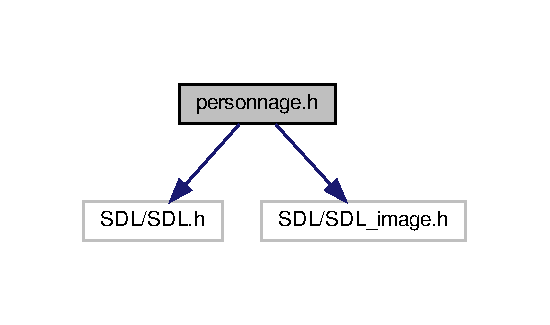
\includegraphics[width=264pt]{personnage_8h__incl}
\end{center}
\end{figure}
This graph shows which files directly or indirectly include this file\+:
\nopagebreak
\begin{figure}[H]
\begin{center}
\leavevmode
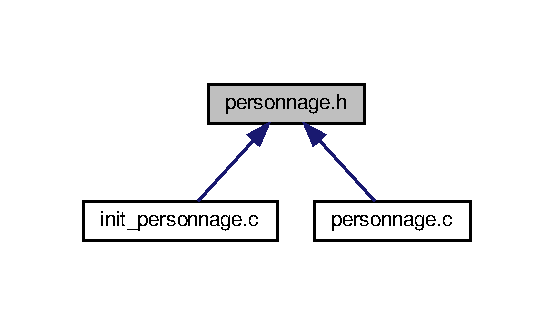
\includegraphics[width=266pt]{personnage_8h__dep__incl}
\end{center}
\end{figure}
\subsection*{Classes}
\begin{DoxyCompactItemize}
\item 
struct \hyperlink{structPersonnage}{Personnage}
\end{DoxyCompactItemize}
\subsection*{Typedefs}
\begin{DoxyCompactItemize}
\item 
typedef struct \hyperlink{structPersonnage}{Personnage} \hyperlink{personnage_8h_ac78ec708d46536e4ce5c5eca5150d4d4}{Player}
\end{DoxyCompactItemize}
\subsection*{Functions}
\begin{DoxyCompactItemize}
\item 
void \hyperlink{personnage_8h_aea858edd1e8f6fcf5c2f55e455ba63e2}{Personnage\+\_\+\+Init} (\hyperlink{structPersonnage}{Personnage} $\ast$p)
\item 
void \hyperlink{personnage_8h_ae662e220210cf8bb89108a9e9f4c3c61}{Personnage\+\_\+\+Render} (\hyperlink{structPersonnage}{Personnage} $\ast$p, S\+D\+L\+\_\+\+Rect r, S\+D\+L\+\_\+\+Surface $\ast$$\ast$screen)
\end{DoxyCompactItemize}


\subsection{Typedef Documentation}
\mbox{\Hypertarget{personnage_8h_ac78ec708d46536e4ce5c5eca5150d4d4}\label{personnage_8h_ac78ec708d46536e4ce5c5eca5150d4d4}} 
\index{personnage.\+h@{personnage.\+h}!Player@{Player}}
\index{Player@{Player}!personnage.\+h@{personnage.\+h}}
\subsubsection{\texorpdfstring{Player}{Player}}
{\footnotesize\ttfamily typedef struct \hyperlink{structPersonnage}{Personnage}  \hyperlink{2eme_01personnage_8h_a14182d75f63f296c0c992296e56a37e1}{Player}}



\subsection{Function Documentation}
\mbox{\Hypertarget{personnage_8h_aea858edd1e8f6fcf5c2f55e455ba63e2}\label{personnage_8h_aea858edd1e8f6fcf5c2f55e455ba63e2}} 
\index{personnage.\+h@{personnage.\+h}!Personnage\+\_\+\+Init@{Personnage\+\_\+\+Init}}
\index{Personnage\+\_\+\+Init@{Personnage\+\_\+\+Init}!personnage.\+h@{personnage.\+h}}
\subsubsection{\texorpdfstring{Personnage\+\_\+\+Init()}{Personnage\_Init()}}
{\footnotesize\ttfamily void Personnage\+\_\+\+Init (\begin{DoxyParamCaption}\item[{\hyperlink{structPersonnage}{Personnage} $\ast$}]{p }\end{DoxyParamCaption})}

\mbox{\Hypertarget{personnage_8h_ae662e220210cf8bb89108a9e9f4c3c61}\label{personnage_8h_ae662e220210cf8bb89108a9e9f4c3c61}} 
\index{personnage.\+h@{personnage.\+h}!Personnage\+\_\+\+Render@{Personnage\+\_\+\+Render}}
\index{Personnage\+\_\+\+Render@{Personnage\+\_\+\+Render}!personnage.\+h@{personnage.\+h}}
\subsubsection{\texorpdfstring{Personnage\+\_\+\+Render()}{Personnage\_Render()}}
{\footnotesize\ttfamily void Personnage\+\_\+\+Render (\begin{DoxyParamCaption}\item[{\hyperlink{structPersonnage}{Personnage} $\ast$}]{p,  }\item[{S\+D\+L\+\_\+\+Rect}]{r,  }\item[{S\+D\+L\+\_\+\+Surface $\ast$$\ast$}]{screen }\end{DoxyParamCaption})}


\hypertarget{personnage2_8c}{}\section{personnage2.\+c File Reference}
\label{personnage2_8c}\index{personnage2.\+c@{personnage2.\+c}}


Testing program.  


{\ttfamily \#include $<$S\+D\+L/\+S\+D\+L.\+h$>$}\newline
{\ttfamily \#include $<$S\+D\+L/\+S\+D\+L\+\_\+image.\+h$>$}\newline
{\ttfamily \#include \char`\"{}personnage2.\+h\char`\"{}}\newline
Include dependency graph for personnage2.\+c\+:
\nopagebreak
\begin{figure}[H]
\begin{center}
\leavevmode
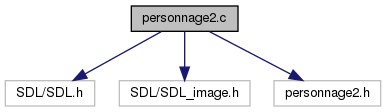
\includegraphics[width=350pt]{personnage2_8c__incl}
\end{center}
\end{figure}
\subsection*{Functions}
\begin{DoxyCompactItemize}
\item 
void \hyperlink{personnage2_8c_a0383a7c926a50b9bbe2357d4f2b98c6e}{Personnage\+\_\+\+Render2} (\hyperlink{structPersonnage}{Personnage} $\ast$p, S\+D\+L\+\_\+\+Rect r, S\+D\+L\+\_\+\+Surface $\ast$$\ast$screen)
\end{DoxyCompactItemize}


\subsection{Detailed Description}
Testing program. 

\begin{DoxyAuthor}{Author}
C Team 
\end{DoxyAuthor}
\begin{DoxyVersion}{Version}
0.\+1 
\end{DoxyVersion}
\begin{DoxyDate}{Date}
juin 10,2020 testing program 
\end{DoxyDate}


\subsection{Function Documentation}
\mbox{\Hypertarget{personnage2_8c_a0383a7c926a50b9bbe2357d4f2b98c6e}\label{personnage2_8c_a0383a7c926a50b9bbe2357d4f2b98c6e}} 
\index{personnage2.\+c@{personnage2.\+c}!Personnage\+\_\+\+Render2@{Personnage\+\_\+\+Render2}}
\index{Personnage\+\_\+\+Render2@{Personnage\+\_\+\+Render2}!personnage2.\+c@{personnage2.\+c}}
\subsubsection{\texorpdfstring{Personnage\+\_\+\+Render2()}{Personnage\_Render2()}}
{\footnotesize\ttfamily void Personnage\+\_\+\+Render2 (\begin{DoxyParamCaption}\item[{\hyperlink{structPersonnage}{Personnage} $\ast$}]{p,  }\item[{S\+D\+L\+\_\+\+Rect}]{r,  }\item[{S\+D\+L\+\_\+\+Surface $\ast$$\ast$}]{screen }\end{DoxyParamCaption})}


%--- End generated contents ---

% Index
\backmatter
\newpage
\phantomsection
\clearemptydoublepage
\addcontentsline{toc}{chapter}{Index}
\printindex

\end{document}
